\chapter{Benchmarking}

\section{Comparing to other database systems}
Comparing our database system with typical database systems is very difficult. We need to prepare same environment.

\subsection{MySQL}
MySQL is free and open-source software under the terms of the GNU General Public License, and is also available under a variety of proprietary licenses. MySQL was owned and sponsored by the Swedish company MySQL AB, which was bought by Sun Microsystems (now Oracle Corporation). MySQL is used by many database-driven web applications, including Drupal, Joomla, phpBB, and WordPress. MySQL is also used by many popular websites, including Facebook,Flickr, MediaWiki, Twitter, and YouTube.

\subsection{PostgreSQL}
PostgreSQL also known as Postgres, is a free and open-source relational database management system emphasizing extensibility and SQL compliance. It was originally named POSTGRES, referring to its origins as a successor to the Ingres database developed at the University of California, Berkeley. In 1996, the project was renamed to PostgreSQL to reflect its support for SQL. After a review in 2007, the development team decided to keep the name PostgreSQL.PostgreSQL features transactions with Atomicity, Consistency, Isolation, Durability (ACID) properties, automatically updatable views, materialized views, triggers, foreign keys, and stored procedures. It is designed to handle a range of workloads, from single machines to data warehouses or Web services with many concurrent users. It is the default database for macOS Server, and is also available for Linux, FreeBSD, OpenBSD, and Windows.

\subsection{Environment}
We compare MySQL and PostgresSQL with our p2p database system. These database systems run virtualized in Docker containers on hardware with 4 core's processor Intel Pentium G4560 3.50GHz and 16GB of RAM. On another hardware we starts clients, that connects to these database systems a preforms queries. Than we measure average queries per seconds that clients execute. Clients are written in javascript with official node.js connectors for MySQL\footnote{\url{https://www.npmjs.com/package/mysql}} and PostgreSQL\footnote{\url{https://www.npmjs.com/package/postgres}} and are connected in the LAN with database systems over 1Gb ethernet. Database structure that is used in benchmarks can be seen in Figure \ref{benchDatabaseStructure}. Table \texttt{authors} contains 10000 records and table \texttt{posts} contains 50000 records (each author has 5 posts). Test query for each database system can be seen in Figure \ref{benchQuery}.

\begin{figure}[h]
    \begin{subfigure}{.3\textwidth}
        \begin{lstlisting}[language=SQL,basicstyle=\tiny]
            CREATE TABLE `authors` (
                `id` int(11) PRIMARY KEY,
                `first_name` varchar(50),
                `last_name` varchar(50),
                `email` varchar(100),
                `birthdate` date,
                `added` timestamp,
                PRIMARY KEY (`id`),
                UNIQUE KEY `email` (`email`)
            );

            CREATE TABLE `posts` (
                `id` int(11) PRIMARY KEY,
                `author_id` int(11),
                `title` varchar(255),
                `description` varchar(500),
                `content` text,
                `date` date,
                PRIMARY KEY (`id`)
            );
        \end{lstlisting}
        \caption{MySQL}
    \end{subfigure}%
    \begin{subfigure}{.3\textwidth}
        \begin{lstlisting}[language=SQL,basicstyle=\tiny]
            CREATE TABLE authors (
                id serial PRIMARY KEY,
                first_name varchar(50),
                last_name varchar(50),
                email varchar(100),
                birthdate date,
                added timestamp
            );

            CREATE TABLE posts (
                id serial PRIMARY KEY,
                author_id integer,
                title varchar(255),
                description varchar(500),
                content text,
                date date
            );
        \end{lstlisting}
        \caption{PostgreSQL}
    \end{subfigure}
    \begin{subfigure}{.3\textwidth}
        \begin{lstlisting}[language=python,basicstyle=\tiny]
            class Author {
                @PrimaryKey() id: number;
                first_name: string;
                last_name: string;
                email: string;
                @Index() birthdate: Date;
                added: Date;
            }

            class Post {
                @PrimaryKey() id: number;
                author_id: number;
                title: string;
                description: string;
                content: string;
                date: Date;
            }
        \end{lstlisting}
        \caption{Our database system}
    \end{subfigure}
    \caption{Database structures for benchmarking}
    \label{benchDatabaseStructure}
\end{figure}


\begin{figure}[h]
    \begin{subfigure}{.3\textwidth}
        \centering
        \begin{lstlisting}[language=SQL,basicstyle=\tiny]
            SELECT * FROM authors 
            JOIN posts ON 
            posts.author_id=authors.id  
            WHERE authors.id=
              (SELECT 
                FLOOR(RAND() * 10001 + 1));
        \end{lstlisting}
        \caption{MySQL}
    \end{subfigure}%
    \begin{subfigure}{.3\textwidth}
        \centering
        \begin{lstlisting}[language=SQL,basicstyle=\tiny]
            SELECT * FROM authors 
            JOIN posts ON 
            posts.author_id=authors.id  
            WHERE authors.id=
              (SELECT 
                floor(random() * 10001 + 1)) ;
        \end{lstlisting}
        \caption{PostgreSQL}
    \end{subfigure}
    \begin{subfigure}{.3\textwidth}
        \centering
        \begin{lstlisting}[language=python,basicstyle=\tiny]
            new Author()
            .where("id")
            .equal(
                Math.floor(
                    Math.random() * 10001) + 1)
            .first();
        \end{lstlisting}
        \caption{Our database system}
    \end{subfigure}
    \caption{Test query}
    \label{benchQuery}
\end{figure}


\subsection{Single connected client}
With a single connected client PostgreSQL can make more than 250 queries per second and MySQL 70 queries per second. Our database system is far behind with up to 20 queries per second (see Figure \ref{bench1per}). We can see that our database system builds cache, and performance increases by time. With only a single connected client there is no advantage of p2p network. CPU usage with a single connected client is for MySQL and PostgreSQL same - about 20\% (see Figure \ref{bench1cpu}). For our database system it is only 3\% due to lots of IO operations. 

\begin{figure}[h]
    \begin{subfigure}{.5\textwidth}
        \centering
        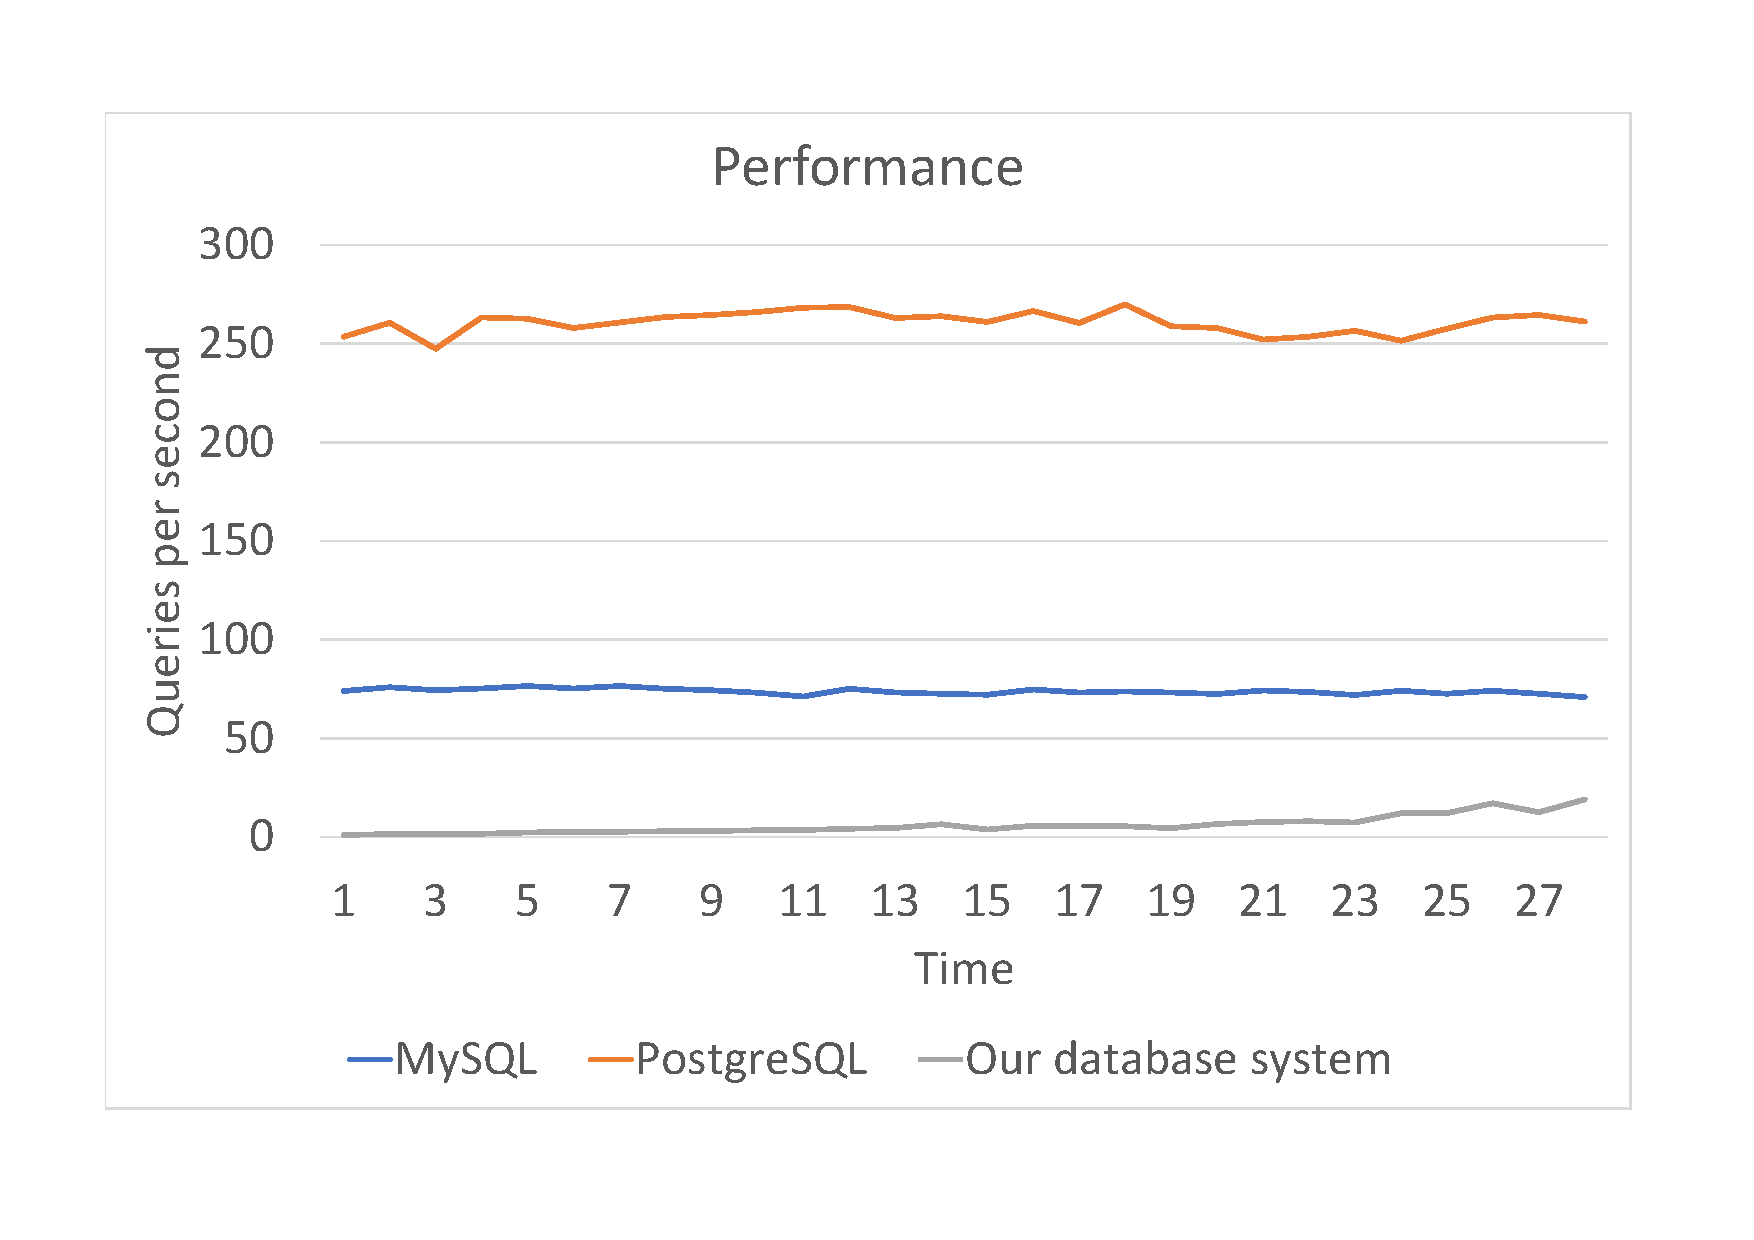
\includegraphics[trim={1.78cm 2cm 2.08cm 1cm},clip,width=1.0\linewidth]{excel/1per.pdf}
        \caption{Performance}
        \label{bench1per}
    \end{subfigure}
    \begin{subfigure}{.5\textwidth}
        \centering
        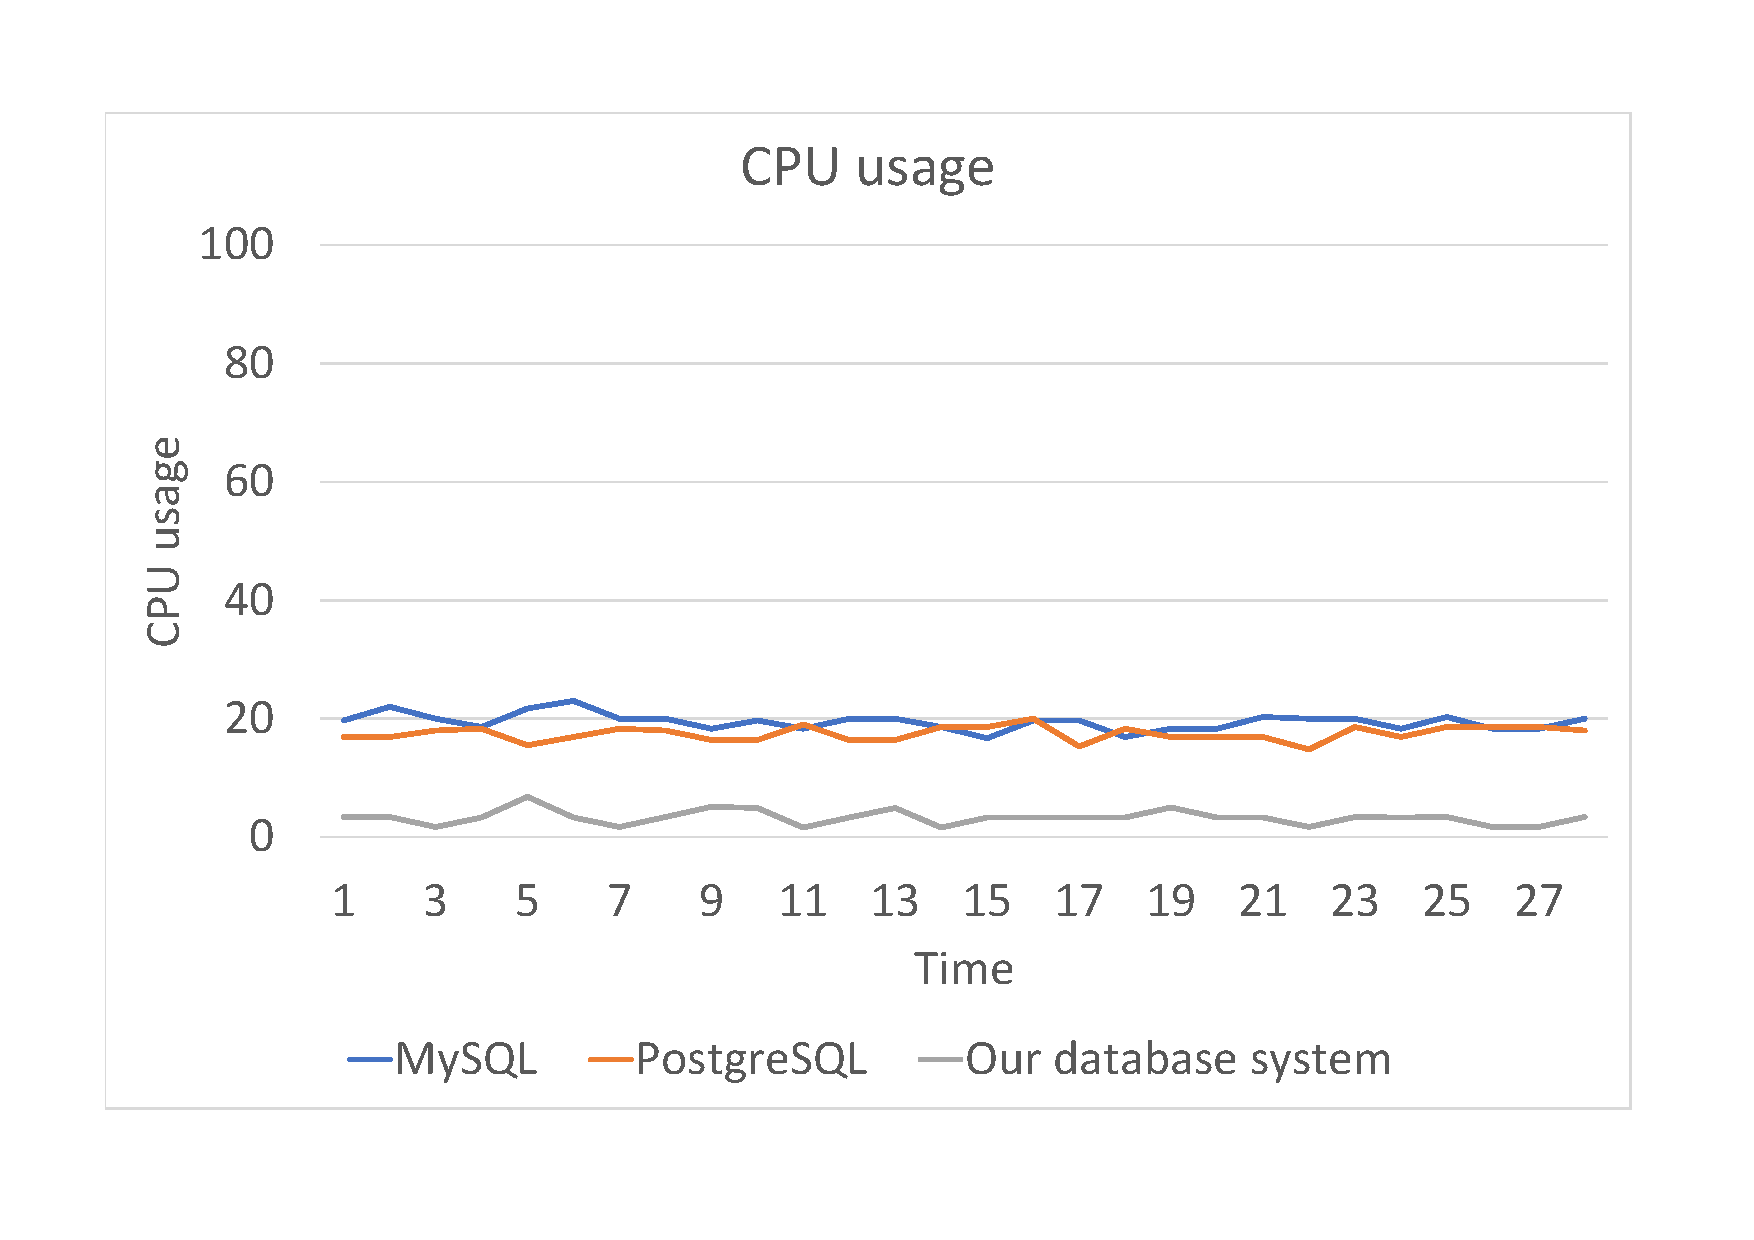
\includegraphics[trim={1.78cm 2cm 2.08cm 1cm},clip,width=1.0\linewidth]{excel/1cpu.pdf}
        \caption{CPU usage with}
        \label{bench1cpu}
    \end{subfigure}
    \caption{Single connected client benchmark plots}
\end{figure}



\subsection{20 connected clients}
With 20 connected clients, PostgreSQL performance dropped to 50 queries per seconds and MySQL to 10 queries per seconds. At the end of benchmarking, our database system is more powerful than PostgreSQL and MySQL, because data gets distributed to clients (see \ref{bench20per}). Our database system also requires less processor time thanks to p2p network. Data are not obtained only from the server (as opposed to MySQL and PostgreSQL) but also from other clients. Thanks to this our system only using less than 20\% CPU power (see Figure \ref{bench20cpu}).

\begin{figure}[h]
    \begin{subfigure}{.5\textwidth}
        \centering
        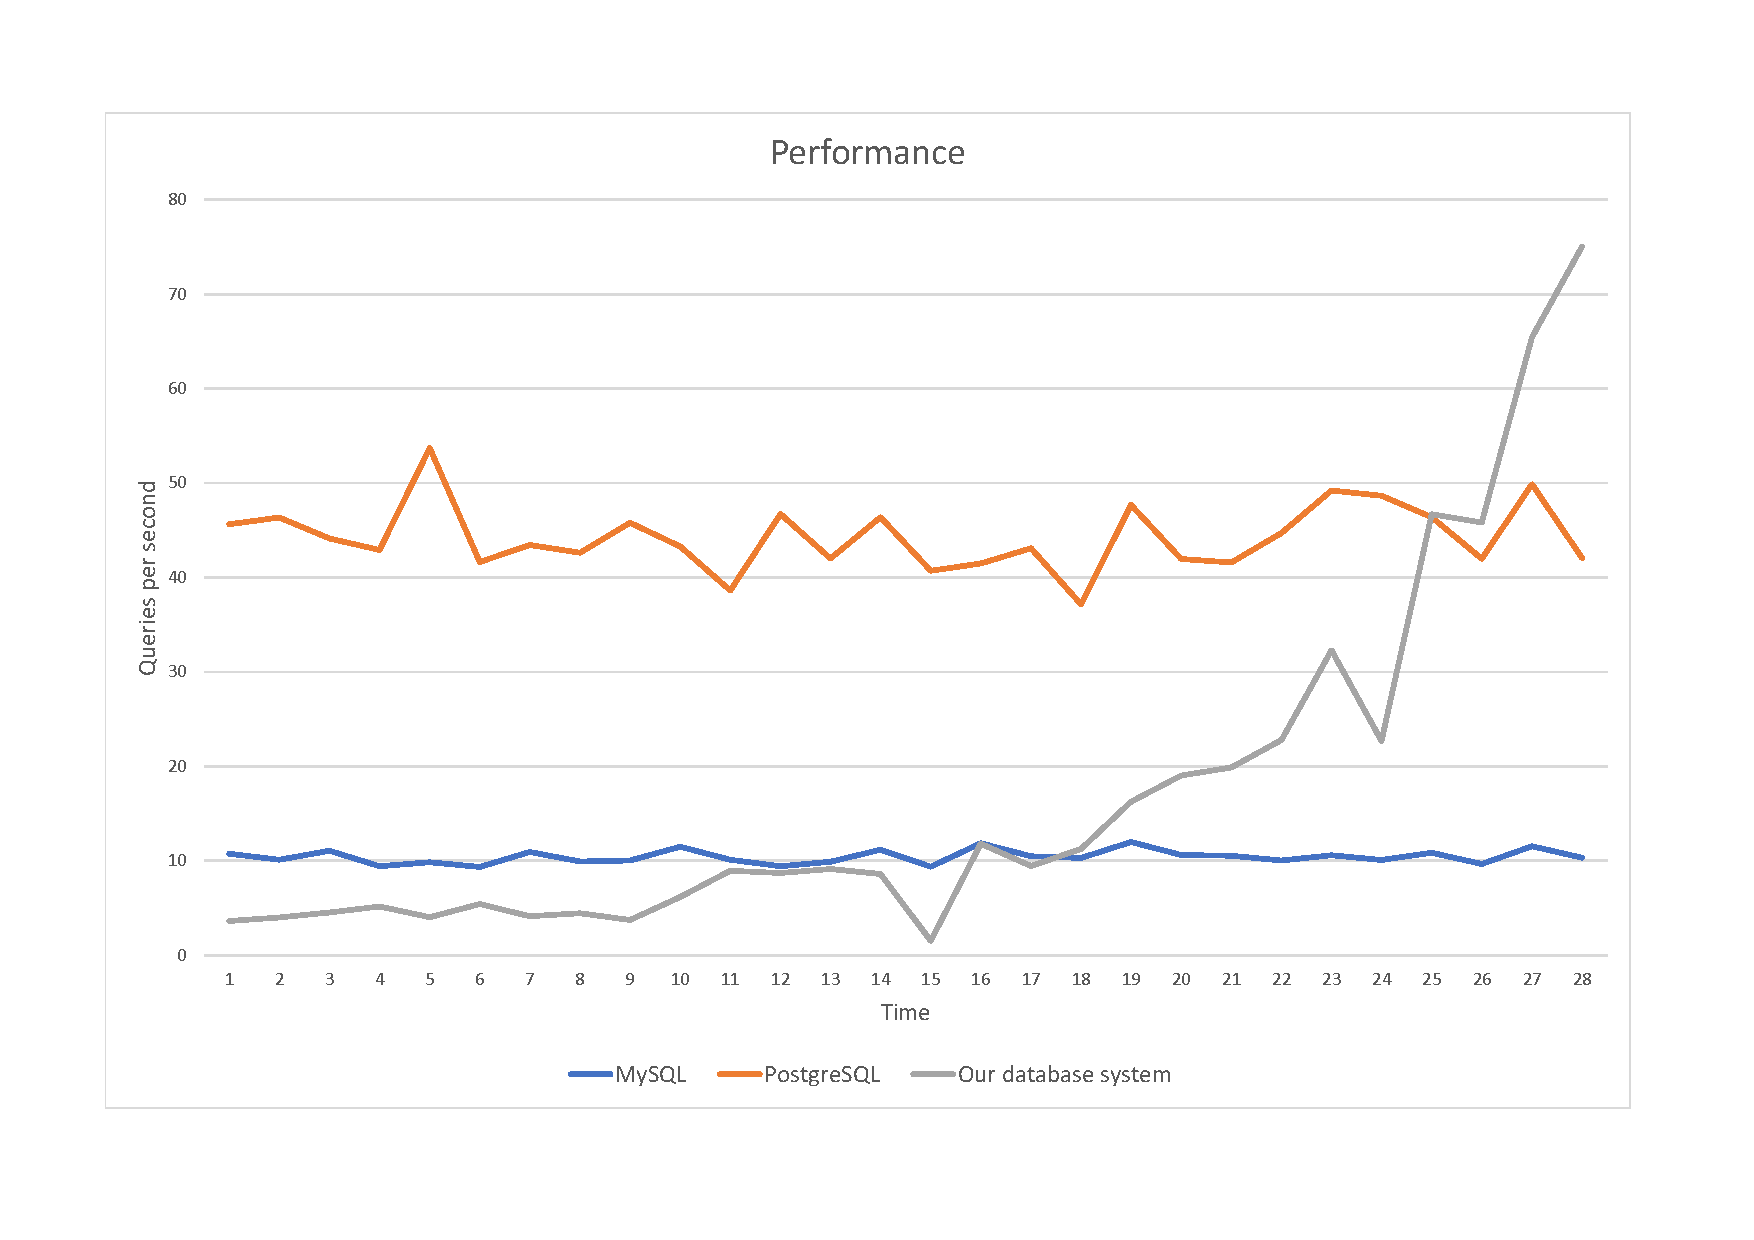
\includegraphics[trim={1.78cm 2cm 2.08cm 1cm},clip,width=1.0\linewidth]{excel/20per.pdf}
        \caption{Performance}
        \label{bench20per}
    \end{subfigure}
    \begin{subfigure}{.5\textwidth}
        \centering
        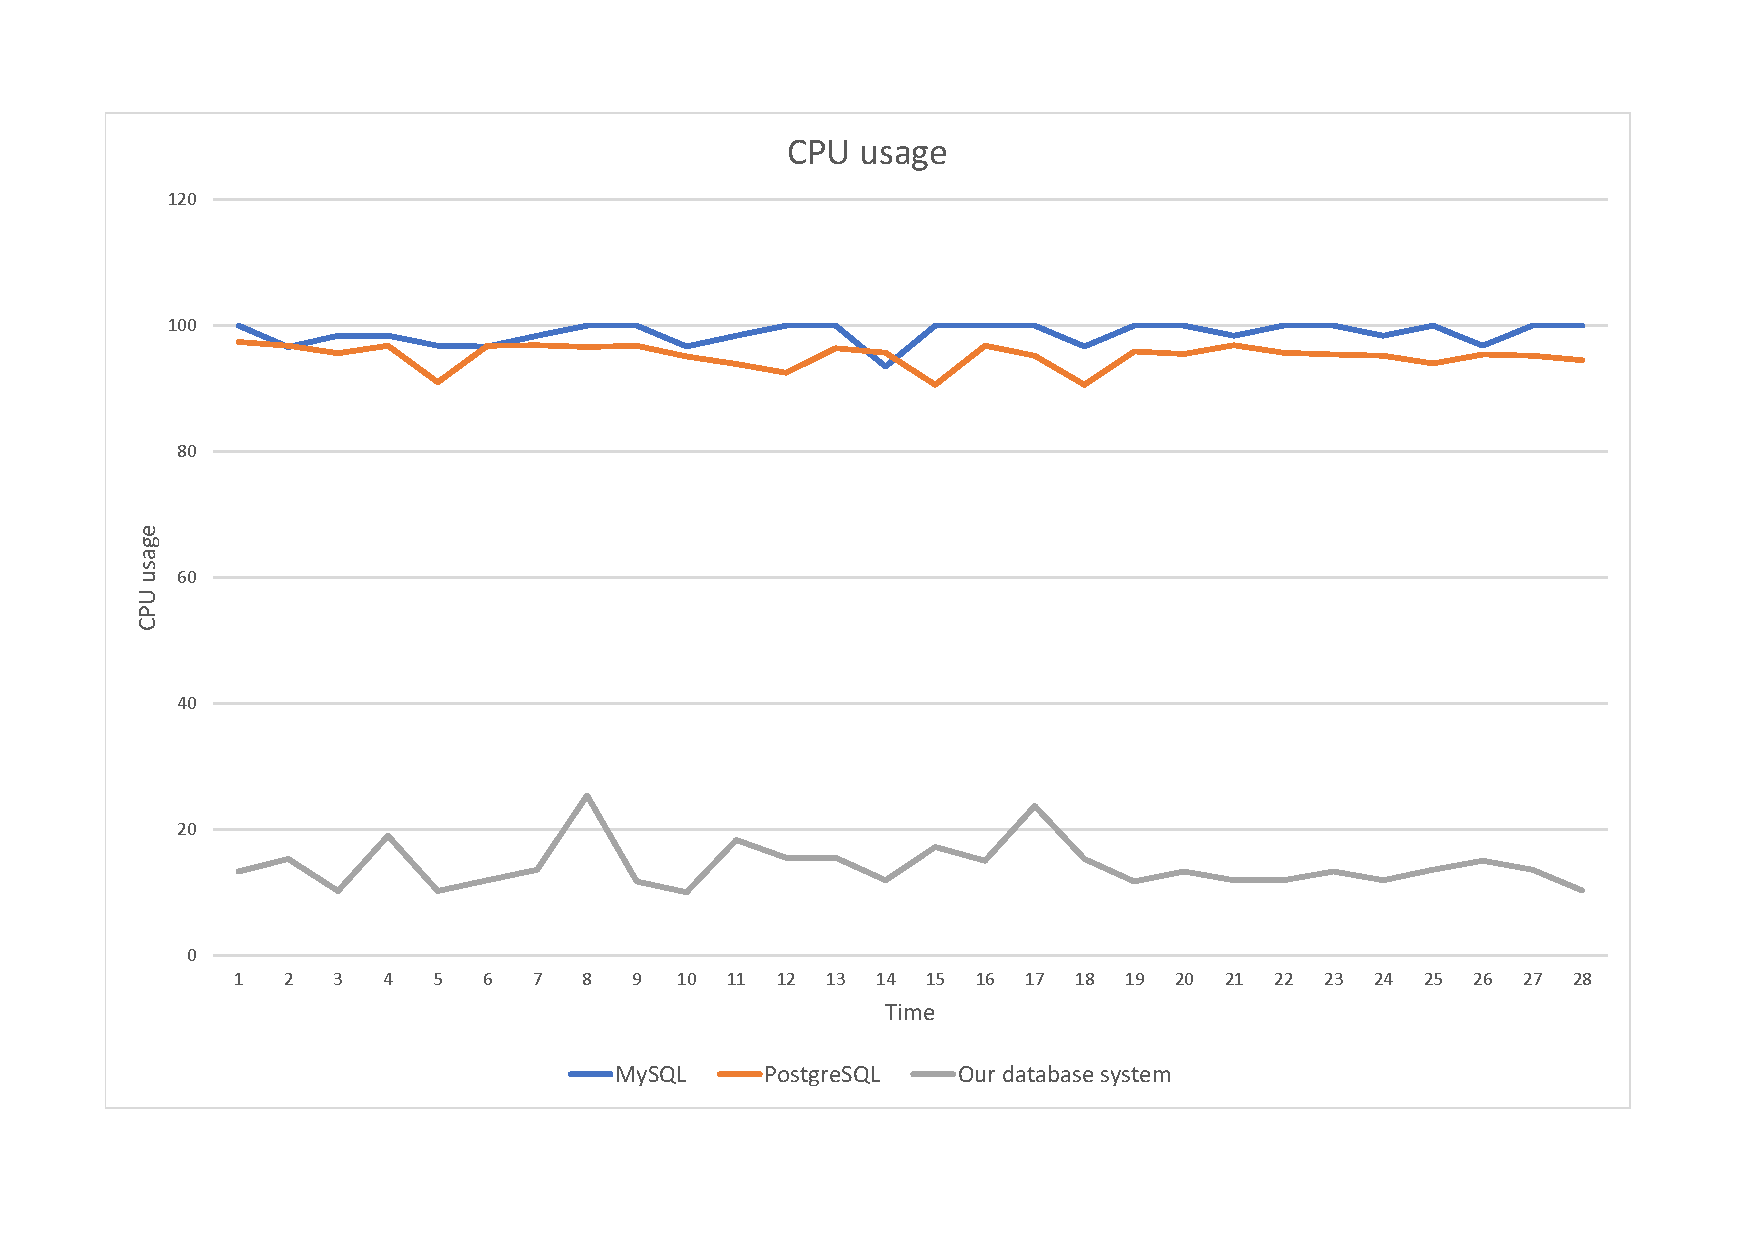
\includegraphics[trim={1.78cm 2cm 2.08cm 1cm},clip,width=1.0\linewidth]{excel/20cpu.pdf}
        \caption{CPU usage with}
        \label{bench20cpu}
    \end{subfigure}
    \caption{20 connected clients benchmark plots}
\end{figure}


\subsection{80 connected clients}
With 80 connected clients, our database system outperforms MySQL and PostgreSQL after few seconds. Every client of our database system performs 100 queries per second. PostgreSQL client performs only 10 queries per second and MySQL only 2 queries per second (see \ref{bench80per}). CPU usage is in our database system also very low. At the beginning, when content is not distributed on the clients, the central node uses 60 percents of CPU but it decreases over time (see \ref{bench80cpu}).


\begin{figure}[h]
    \begin{subfigure}{.5\textwidth}
        \centering
        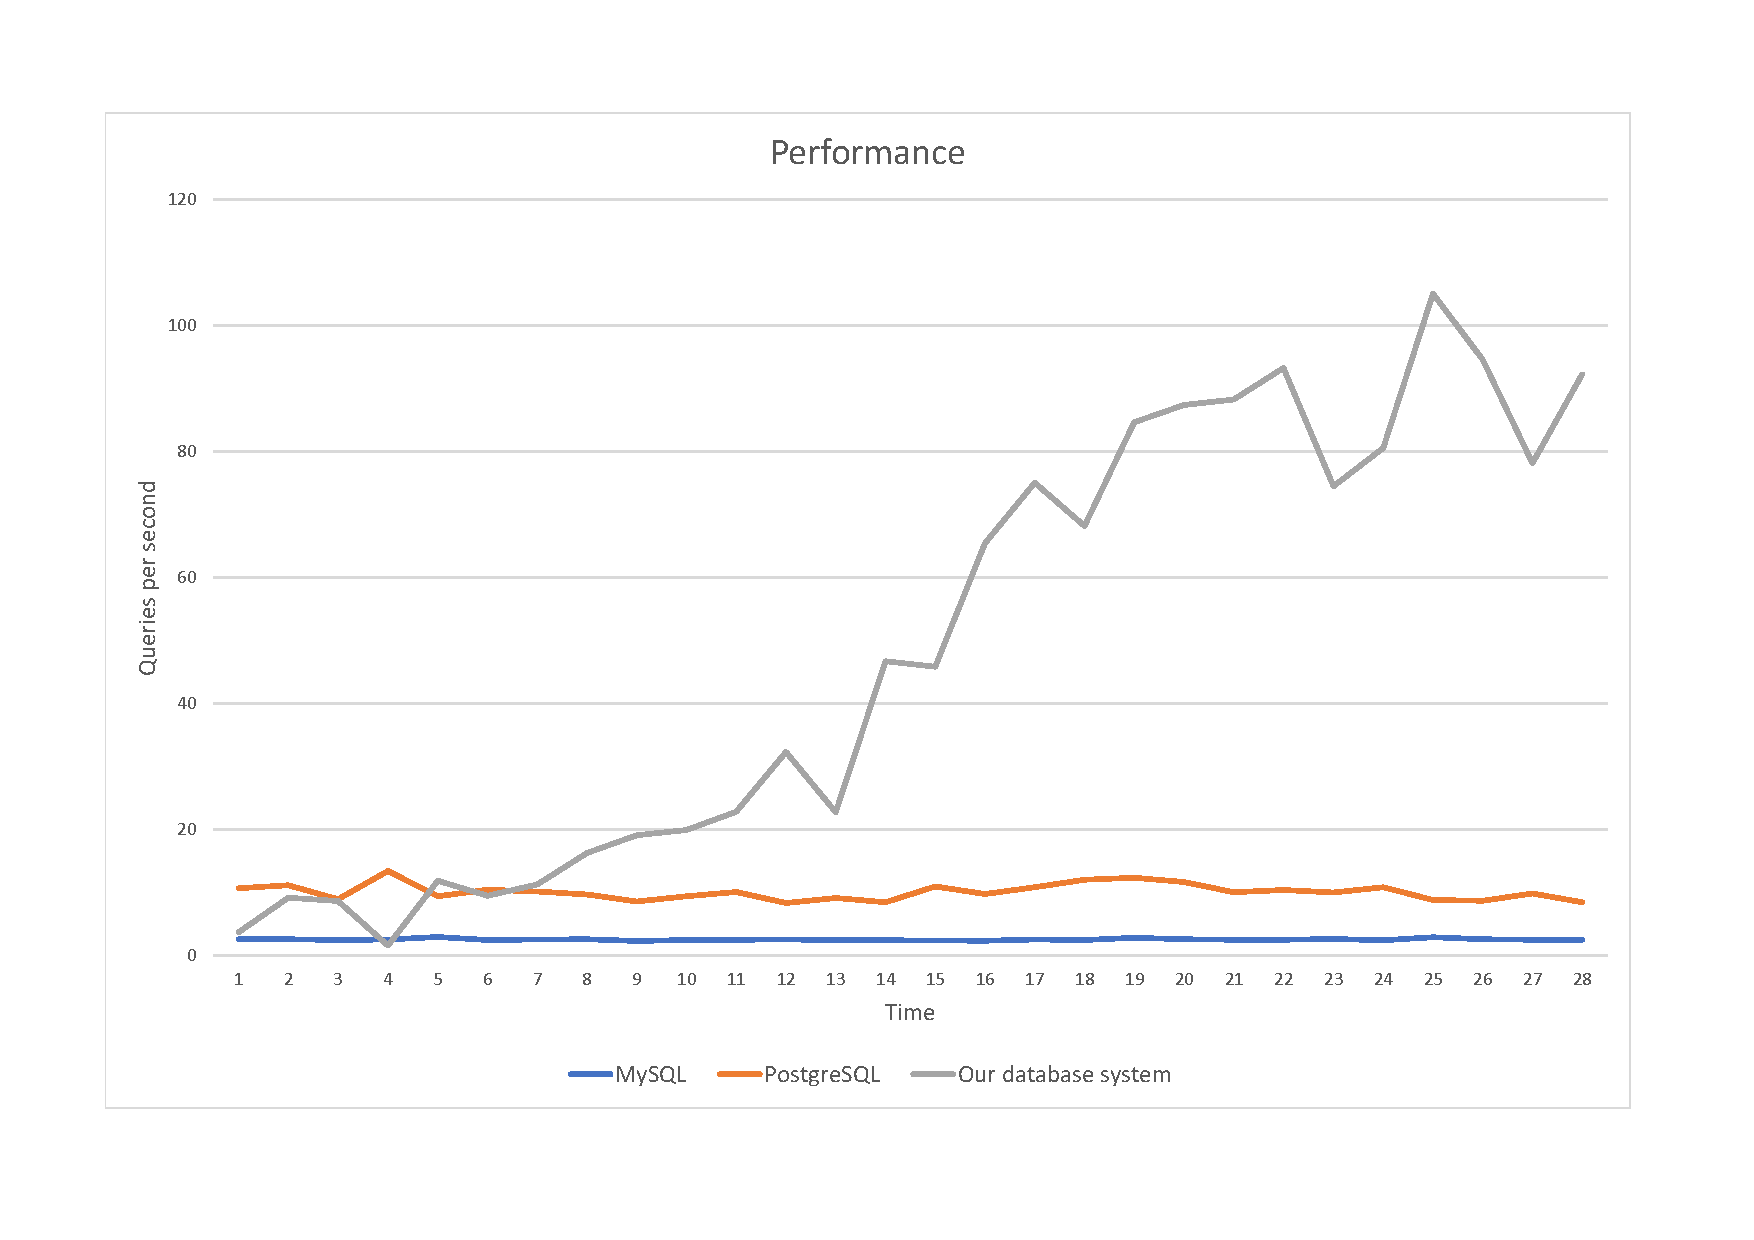
\includegraphics[trim={1.78cm 2cm 2.08cm 1cm},clip,width=1.0\linewidth]{excel/80per.pdf}
        \caption{Performance}
        \label{bench80per}
    \end{subfigure}
    \begin{subfigure}{.5\textwidth}
        \centering
        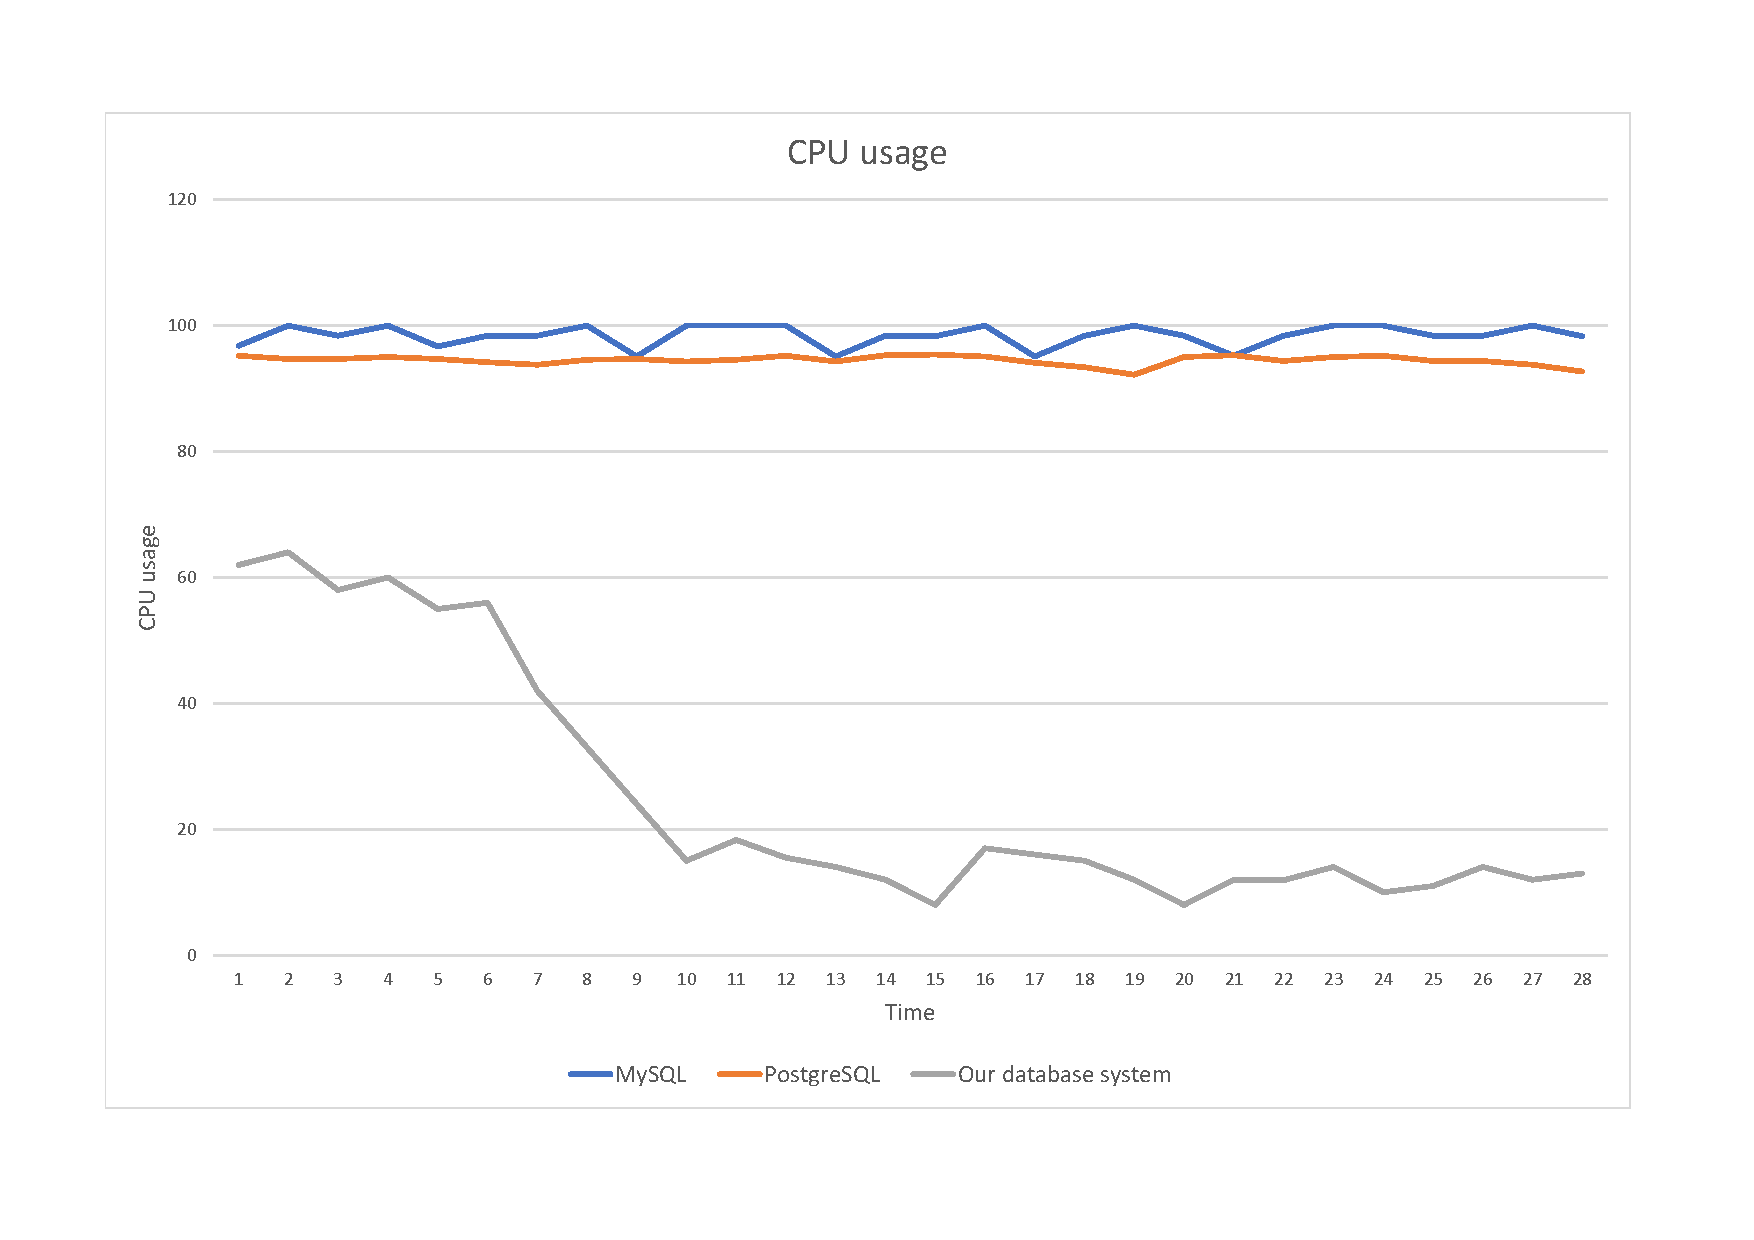
\includegraphics[trim={1.78cm 2cm 2.08cm 1cm},clip,width=1.0\linewidth]{excel/80cpu.pdf}
        \caption{CPU usage with}
        \label{bench80cpu}
    \end{subfigure}
    \caption{80 connected clients benchmark plots}
\end{figure}


\subsection{150 connected clients}
To connects more than 100 clients to the PostgreSQL, we need to change  default PostgreSQL setting for maximum connections. Our system can handle 150 clients very well (opposite to MySQL and PostgreSQL). Each client connected to our database system can make up to 150 queries per second, and it increases by the time (see \ref{bench150per}). For the first seconds, CPU usage on the central node is high (near 100\%), but it decreases over the time (see \ref{bench150cpu}).

\begin{figure}[h]
    \begin{subfigure}{.5\textwidth}
        \centering
        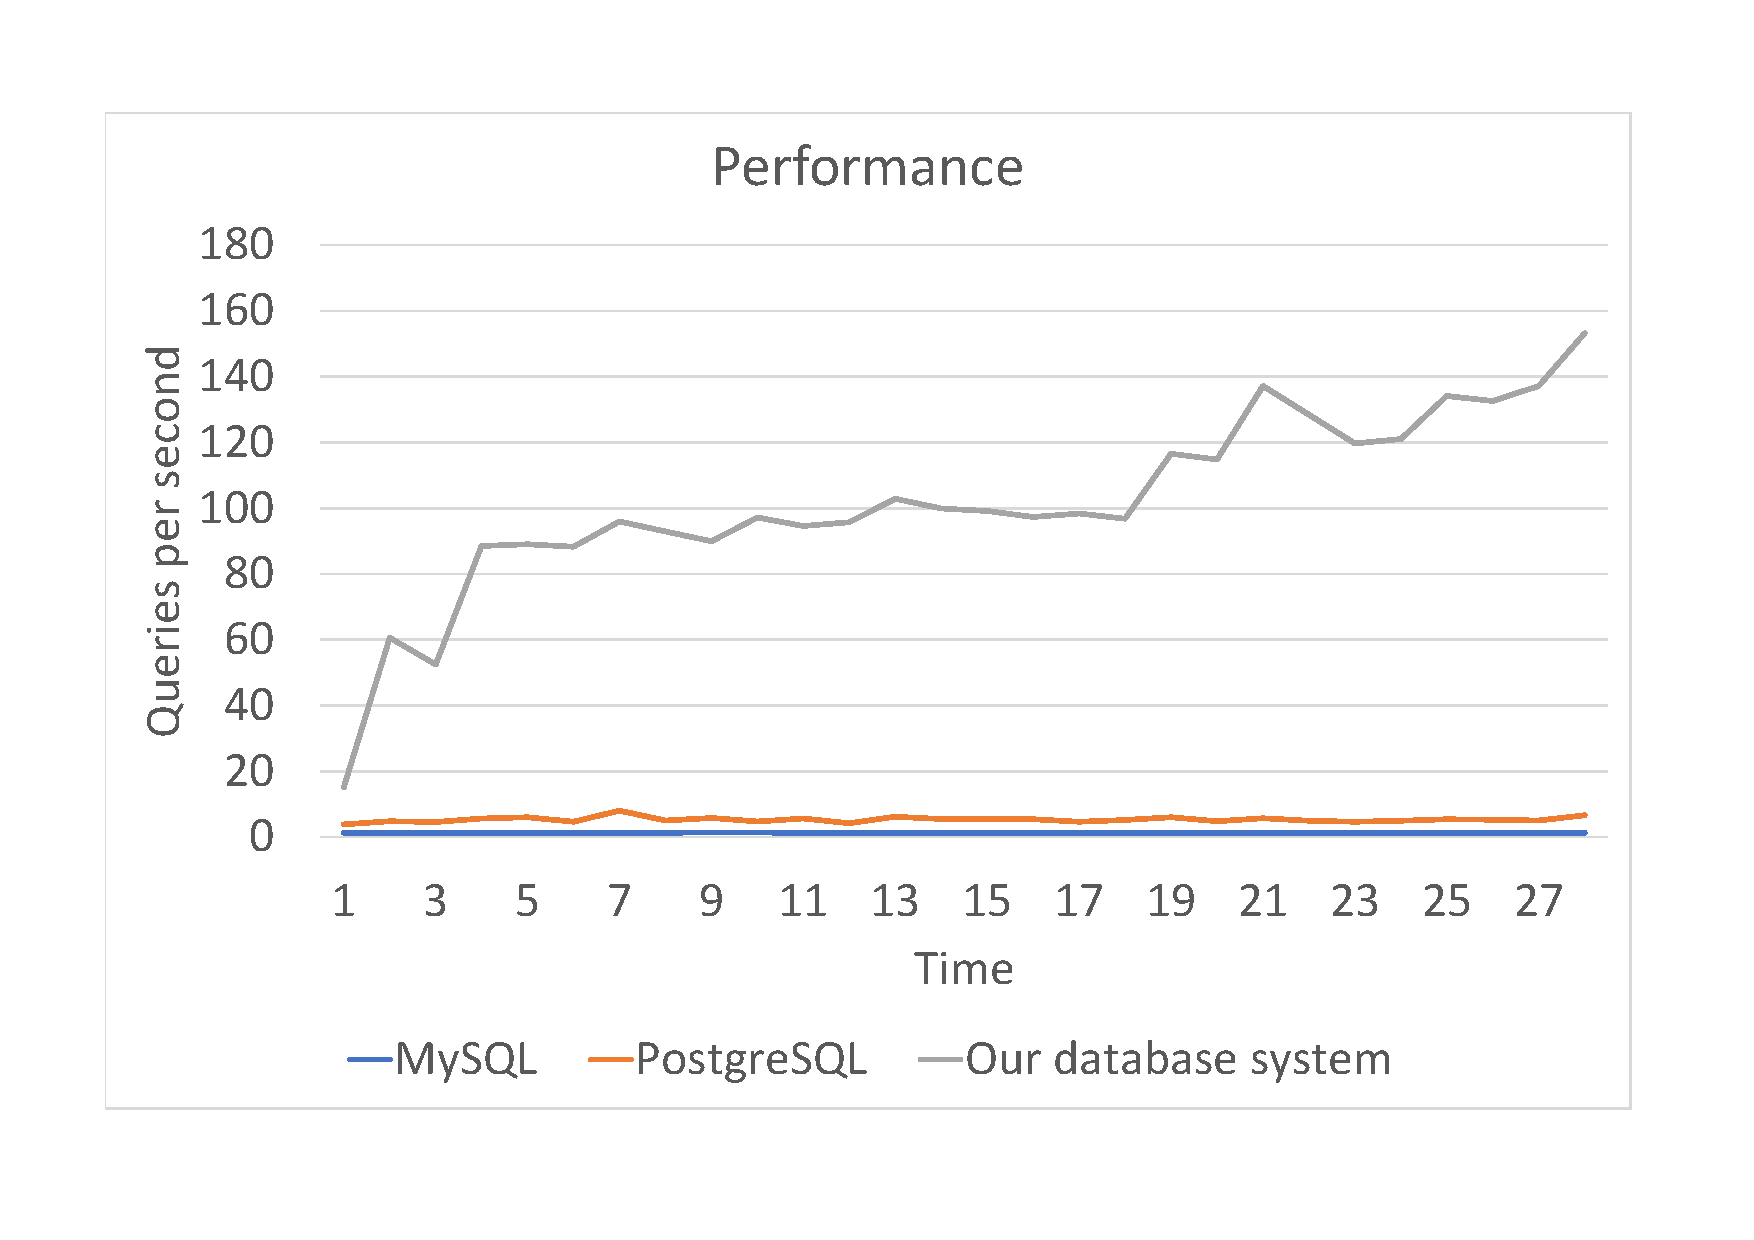
\includegraphics[trim={1.78cm 2cm 2.08cm 1cm},clip,width=1.0\linewidth]{excel/150per.pdf}
        \caption{Performance}
        \label{bench150per}
    \end{subfigure}
    \begin{subfigure}{.5\textwidth}
        \centering
        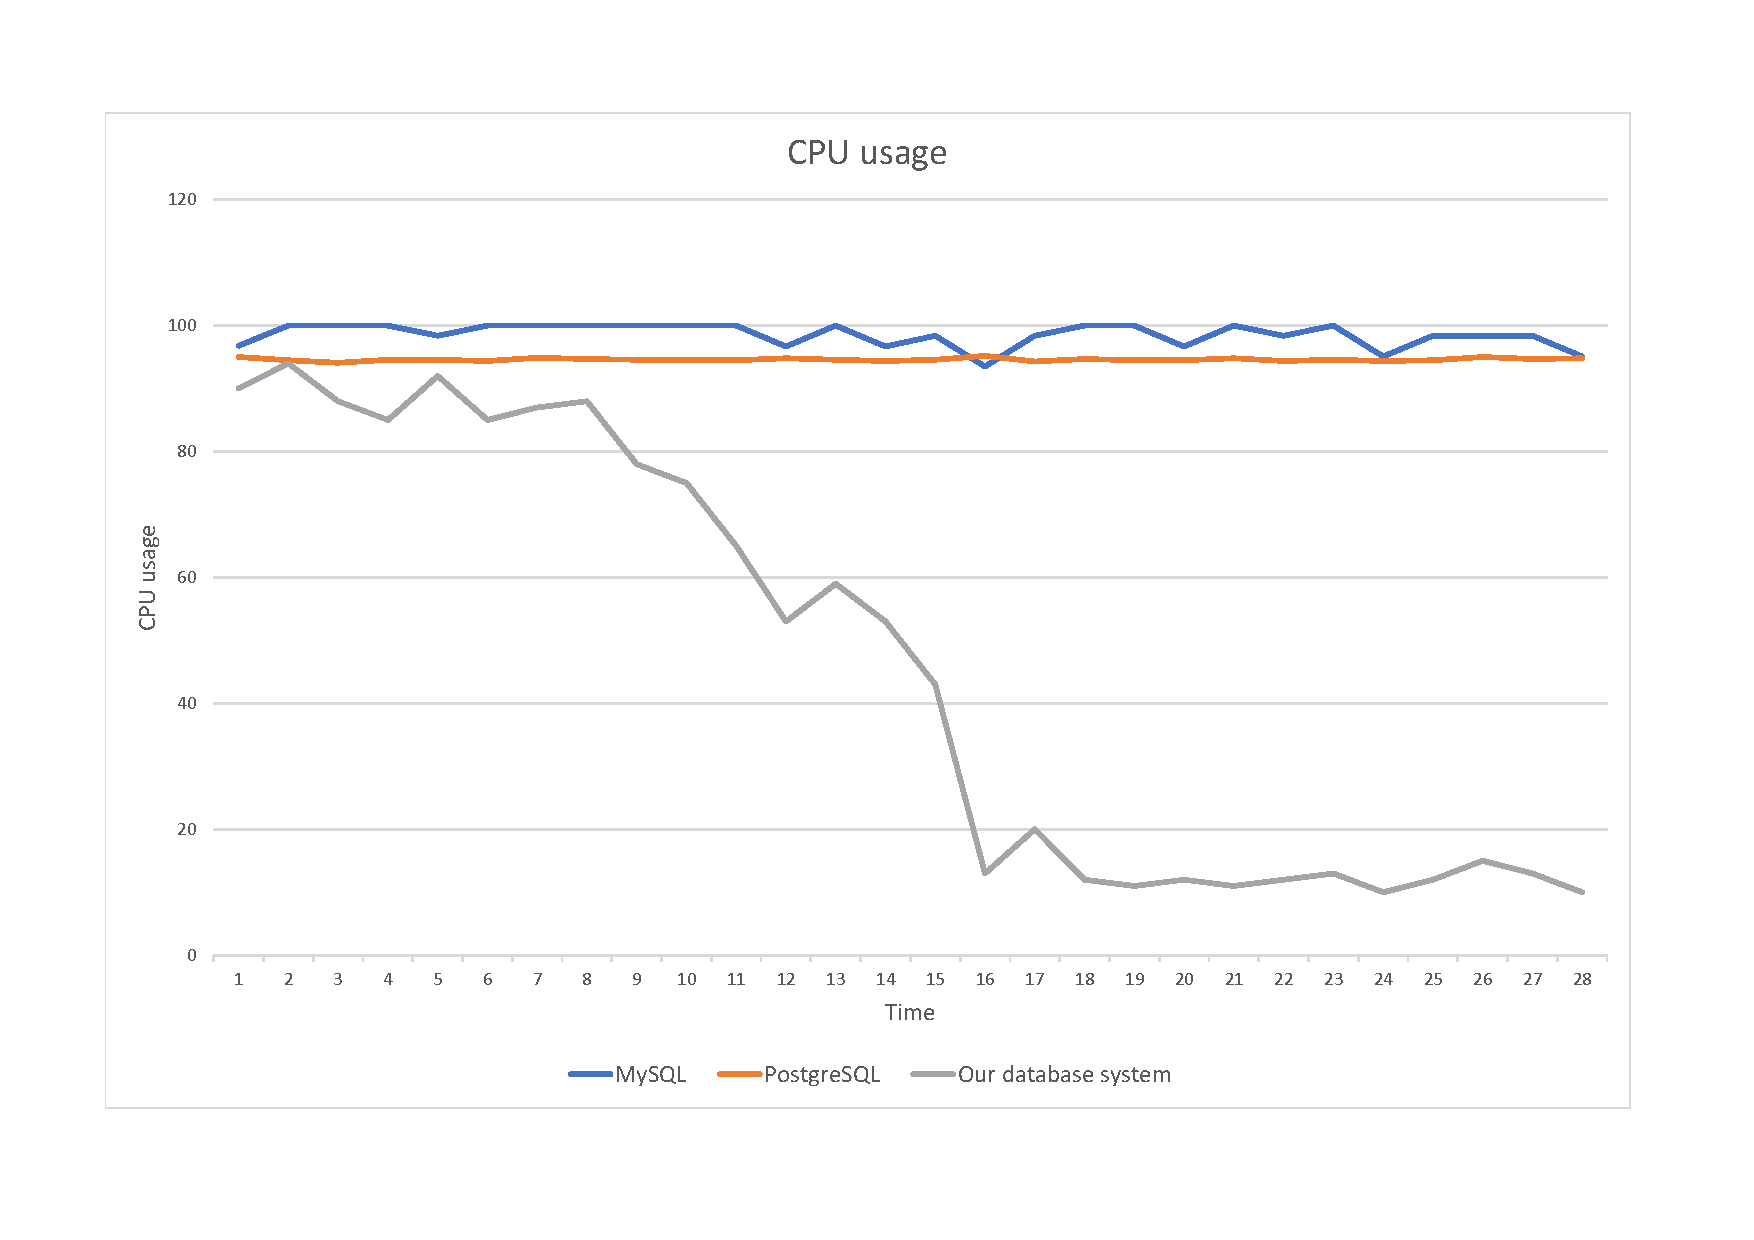
\includegraphics[trim={1.78cm 2cm 2.08cm 1cm},clip,width=1.0\linewidth]{excel/150cpu.pdf}
        \caption{CPU usage with}
        \label{bench150cpu}
    \end{subfigure}
    \caption{150 connected clients benchmark plots}
\end{figure}

\subsection{Benchmark conclusion}
We can see that with more than 20 connected clients, our database system became more effective than traditional ones. Thanks to IPFS and its p2p network, a content of the database is distributed on the clients. This reduces load on central node.

\section{Comparing with blockchain explorers}


\subsection{Blockbook}
Blockbook\footnote{\url{https://github.com/trezor/blockbook}} is a blockchain indexer for Trezor Wallet\footnote{\url{https://wallet.trezor.io/}}, developed by SatoshiLabs\footnote{\url{https://satoshilabs.com/}}. It currently supports more than 30 coins (and the community implemented some others). For data storage Blockbook is using RocksDB\footnote{\url{https://github.com/facebook/rocksdb/wiki}} developed by Facebook, which is a NoSQL database that stores only key-value pairs. Blockbook is providing fast API for accessing blocks, addresses and transactions. Main limitations of blockbook:
\begin{itemize}
    \item \textbf{Not distributed} (client-server architecture) - problem with scaling for more users. 
    \item \textbf{Not a SQL database} - it does not have a relational data model, it does not support SQL queries, and it has no support for indexes.
    \item \textbf{Single-Process} - only a single process (possibly multi-threaded) can access a particular database at a time.
\end{itemize}

\todo{Najprv je potrebne synchronizovat cely blockchain aby som mohol uskutocnit merania}
\subsection{Writing}

\subsection{Reading}


\subsection{Filtering}